\documentclass[conference,letterpaper]{IEEEtran}
\usepackage{amsmath,amssymb}
\usepackage{graphicx}
\usepackage{booktabs,array}
\usepackage{tikz}
\usetikzlibrary{arrows.meta,positioning,shapes.geometric,calc}
\usepackage[hidelinks]{hyperref}
\urlstyle{same}
\newcommand{\cmode}{C-MODE}
\newcommand{\JSD}{\operatorname{JSD}}
\newcommand{\ind}{\mathbf{1}}
\newcounter{algorithm}
\tikzset{box/.style={draw,rounded corners=2pt,align=center,font=\footnotesize,minimum height=6mm,text width=31mm,inner sep=3pt},
 decision/.style={draw,diamond,aspect=2.3,align=center,font=\scriptsize,inner sep=1pt,text width=22mm},
 arr/.style={-{Latex[length=1.5mm]},thin}}
\title{GenRaga: Constrained Multi-Objective Differential Evolution for Carnatic Melody Generation}

\author{\IEEEauthorblockN{Shrinidhi Maheshwaran}
\IEEEauthorblockA{\textit{Department of Computer Science and Engineering} \\
\textit{Amrita School of Computing, Coimbatore}\\
\textit{Amrita Vishwa Vidyapeetham}, Ettimadai, India\\
cb.sc.p2cse25033@cb.students.amrita.edu}
\and
\IEEEauthorblockN{Ritwik M}
\IEEEauthorblockA{\textit{Department of Computer Science and Engineering} \\
\textit{Amrita School of Computing, Coimbatore}\\
\textit{Amrita Vishwa Vidyapeetham}, Ettimadai, India\\
\href{mailto:m_ritwik@cb.amrita.edu}{m\_ritwik@cb.amrita.edu}}
}

\begin{document}
\maketitle

\begin{abstract}
Authentic composition of Carnatic music requires strict constraints of grammar, microtonality and rhythmic cycles. In South Indian classical music melody is composed with respect to constraints of grammar (raga), microtonality (gamaka) and rhythmic cycle (tala). This paper proposes GenRaga, an evolutionary approach to music generation, formulating the problem of melody composition as a Constrained Multi-Objective Differential Evolution (C-MODE) problem in the context of phrase cell corpus composition. We compose grammar move graphs of seven core ragas (Mohanam, Kalyani, Abhogi, Begada, Sahana, Saveri, Sri) for 705 tracks including both audio and pitch data for 103 raga classes. Melodies are composed by generating sequences of rhythmic akshara cells, and then optimized using differential vectors in a 9-dimensional feature space using mutation, nearest neighbour constrained legal snapping, constraint join fixing and NSGA-II non-dominated sorting for five competing musical proxy objectives. Continuous audio is generated by combining the generated skeletal pitch data with microtonal contour residual data extracted from 27,731 notes from 28 vocal performances using dynamic time warping. C-MODE performs consistently better than random walks under balanced constraints (up to 30.2\% improvement in Begada, 29.8\% in Sri) with 100\% valid structures. C-MODE avoids genetic drift under strict constraints, outperforming all weighted sum genetic algorithms (100\% success rate). Melodies are composed with median pitch error of 0.824 cents and an internal classifier (42 raga classes) has 94.4\% accuracy.
\end{abstract}

\begin{IEEEkeywords}
Carnatic music, constrained optimisation, differential evolution, multi-objective optimisation, algorithmic composition, gamaka synthesis, music information retrieval.
\end{IEEEkeywords}

\section{Introduction}
\subsection{Background and Motivation}
Deep generative models can produce interesting audio textures using text or symbolic inputs~\cite{copet2023}. However, statistical sampling cannot ensure any formal grammar is followed in the output. Whilst we may generate audio textures with typical string or vocal characteristics for text prompts such as ``Carnatic Kalyani in Adi Tala'', we cannot ensure that the scale is legal or that there are no illegal intervals. We cannot use statistical black box decoders to generate music as we need it to be correctly structured.

Carnatic music provides a well structured problem to work with. It has three highly interlinked components:
\begin{itemize}
    \item \textbf{Raga (Melodic Grammar):} Rules are set for ascending and descending the scale (\textit{arohana/avarohana}). Rules are also set for which illegal (\textit{varjya}) intervals can be used, which notes to rest on (\textit{vadi/samvadi}) and which melodic motifs (\textit{prayoga}) to use.
    \item \textbf{Gamaka (pitch continuity):} Swara in Carnatic music includes many aspects of ornamentation such as microtonal glide, oscillation and inflection depending on the phrase~\cite{gamaka2022}.
    \item \textbf{Tala (rhythmic grammar):} Rhythm is divided into strict time cycles (\textit{avartanams}). These contain irregular rhythm units (\textit{angas}) and subdivisions of beats (\textit{aksharas}). Often music will need to start on specific off beats (\textit{eduppu}).
\end{itemize}
The discrete equal tempered western system does not include all of these features.

\subsection{Problem Statement and Research Gap}
Evolutionary algorithms can be a useful tool for generation of music based on rules with objective functions imposing constraints related to the domain in the combinatorial search space~\cite{herremans2013,majidi2022,mcintyre1994}. Genetic algorithms were used for generation of counterpoint in Western music~\cite{herremans2012,deprisco2020} and Hindustani note sequences~\cite{shukla2023}. However, existing evolutionary symbolic approaches cannot handle continuous gamaka curves and cyclic tala. Existing evolutionary approaches applied for Indian music were highly dependent on Markov Transition Probability Matrices of order 1~\cite{shukla2023}, making generation of multi-octave phrases impossible.

A recently suggested evolutionary approach was proposed by Prakash \textit{et al.}~\cite{prakash2026} for generation of novel parent-child frameworks of Janya raga using binary scale chromosomes. But this is the problem of generation of complete and expressive melodies inside raga with constraints on scales, rhythmic phrases and microtonal curves.

\subsection{Research Questions and Contributions}
The following research questions were investigated:
\begin{itemize}
    \item \textit{RQ1:} What is the effect of strict and balanced constraints on graph connectivity and exploration ability of melodies?
    \item \textit{RQ2:} How the performance of Pareto based Differential Evolution algorithm (\cmode) compares to random walks and weighted sum genetic algorithms with a strict budget of candidate evaluations?
    \item \textit{RQ3:} How well pitch accuracy and raga classification metrics can be used to measure fidelity of the generated music. What are weaknesses of automated proxies?
\end{itemize}

Our contributions are:
\begin{enumerate}
    \item We proposed a framework of tokenization of real Carnatic compositions into rhythmic cells, transition legality within all seven base ragas and combination of symbolic search with gamaka curves obtained from recordings.
    \item We developed \cmode, the version of Differential Evolution which uses 9 dimensional standardized cell features space with discrete snapping of legal transitions and NSGA-II Pareto selection.
    \item We experimented with all seven base ragas (Mohanam, Kalyani, Abhogi, Begada, Sahana, Saveri, Sri), two constraint types (strict and balanced) and five random seeds. All experiments were conducted with a strict budget of candidate evaluations (3,660 evaluations).
    \item We give a thorough analysis of comparison between multiple objectives Pareto optimisation and weighted sum scalarisation. We show the weaknesses of neural net in extrapolation of gamaka curves, transcription and motif identification.
\end{enumerate}

\section{Related Work}
\subsection{Evolutionary and Grammar-Constrained Music Generation}
Evolutionary music composition has stemmed from rule-based genetic algorithms for harmonic counterpoint and motivic interpolation~\cite{mcintyre1994,horner1991,maddox2000}. Early applications focused on four part harmony and species counterpoint with manually defined penalties~\cite{donnelly2011,donnelly2012,phonamnuaisuk1999}. Metaheuristics such as Variable Neighborhood Search were shown to be an effective way of modeling counterpoint rules using sub-score quantification~\cite{herremans2012,herremans2013}. Multi-objective fitness functions based on multiple features have been used for melodic extension and music style imitation in works by Towsey \textit{et al.}~\cite{towsey2001}, Marques \textit{et al.}~\cite{marques2000} and Mati{\'c}~\cite{matic2010}.

Recombinant composition based on corpus statistics were developed in Eigenfeldt~\cite{eigenfeldt2012} and De Prisco \textit{et al.}~\cite{deprisco2020} for harmonizing Bach chorales by using n-gram statistics. Hofmann~\cite{hofmann2015} used Genetic Programming to evolve hierarchical music using tree-based phrases. Hybrid approaches using evolutionary algorithms with neural networks were developed early on by Burton and Vladimirova~\cite{burton1998}. Recently, Farzaneh and Toroghi~\cite{farzaneh2019,farzaneh2020} have used recurrent networks to develop interactive and generative melody algorithms. Multi-objective genetic algorithms were combined with deep learning fitness functions by Majidi and Toroghi~\cite{majidi2022}.

In the improvisation and Jazz domain, real-time interactive genetic algorithms were pioneered by Biles' GenJam~\cite{biles1994,biles2001}. The GenJam system has been extended by Papadopoulos and Wiggins~\cite{papadopoulos1998}, {\"O}zcan and Er{\c{c}}al~\cite{ozcan2008} and Liu and Ting~\cite{liuting2019} using rule-based and machine learning fitness functions. MetaCompose was used for macro-structural affective music generation by Scirea \textit{et al.}~\cite{scirea2017}. Grammatical evolution and Zipf's law information based fitness functions have been used with non-fixed representations by Alfonseca \textit{et al.}~\cite{alfonseca2007}, Manaris \textit{et al.}~\cite{manaris2003}, Loughran \textit{et al.}~\cite{loughran2015} and Ortega \textit{et al.}~\cite{ortega2008}.

Though Differential Evolution (DE) is well known for its ability to perform global optimization on continuous problems~\cite{storn1997}, there are few examples of its application to discrete music composition. Traditional Genetic Algorithms use crossover and mutation which often disrupts melodic structure. We utilise the difference between vectors in DE to guide the selection of discrete phrases within a continuous representation. We also use NSGA-II non-dominated sorting~\cite{deb2002} to maintain a balance between multiple conflicting music objectives without using arbitrary weights~\cite{zitzler2003}.

\subsection{Indian-Classical / Carnatic Generative Systems}
Indian Classical Music has seen algorithmic applications move from rule-based systems to statistical and evolutionary systems. Shukla and Banka~\cite{shukla2023} proposed a hybrid approach using Markov Transition Probability Matrices of order one and genetic search with $\epsilon$-greedy to generate Hindustani raga. This approach was effective at generating simple note transitions but had no quantization of the tala meter and only used single note tokens. No microtonal ornaments were included.

Nandekar \textit{et al.}~\cite{nandekar2021} showed that parent (Melakarta) and child (Janya) ragas in Carnatic music have directional causal relationships when compressed with Lempel-Ziv-Penalty. Prakash \textit{et al.}~\cite{prakash2026} have pioneered the evolutionary development of new Janya raga scales from Melakarta parents using domain specific genetic operators. Our work is different as we are not seeking new raga scales but evolving complete compositions within ragas using rhythmic cells and continuous pitch synthesis.

\subsection{Gamaka Synthesis and Domain Specific Evaluation}
Due to the inability to represent Carnatic music with flat MIDI notes, creating continuous pitch curves is fundamental. A masked latent Convolutional Autoencoder was proposed by Sankaranarayanan and Weinberg~\cite{gamaka2022} to predict continuous pitch from symbolic swara skeletons for the Hathaani robotic violinist. An in-depth study with multi-tempo evaluation was presented in~\cite{gamaka2025}.

Large sets of data are available in the public domain such as the Saraga repository~\cite{saraga2021}. This allows for progress to be made in Computational Ethnomusicology due to their annotated nature. For example, there are audio, pitch and structure annotations. However, it is difficult to evaluate the Indian music that has been generated. General metrics such as Fr{\'e}chet Audio Distance (FAD) or CLAP embeddings do not capture the raga/tala structure of the music, only the timbre. Therefore, we define domain specific metrics such as scale entropy, interval shapes, classifier probabilities and cycle boundary constraints.

\subsection{GenRaga Comparison}
A comparison can be seen in Table~\ref{tab:related}. GenRaga closes the gap between symbolic evolutionary search and empirical search. We compare the constraint topologies with equal computational budget.

\begin{table}[t]
\caption{Systematic comparison to similar work.}
\label{tab:related}
\centering\footnotesize
\begin{tabular}{@{}>{\raggedright\arraybackslash}p{.20\columnwidth}>{\raggedright\arraybackslash}p{.38\columnwidth}>{\raggedright\arraybackslash}p{.32\columnwidth}@{}}
\toprule
System & Core Methodology & Scope \& Limitations\\
\midrule
Shukla et al.~\cite{shukla2023} & Markov TPM + $\epsilon$-greedy GA & Hindustani; flat notes; no tala; single raga.\\
Prakash et al.~\cite{prakash2026} & Constraint-aware GA on binary strings & Evolving Janya scales; no temporal composition.\\
Sankaranar.~\cite{gamaka2022,gamaka2025} & Masked Latent Conv-Autoencoder & Generates gamakas; no symbolic composition.\\
GenRaga (Ours) & Discrete C-MODE (DE + NSGA-II) & Multi-cycle composition; empirical gamakas.\\
\bottomrule
\end{tabular}
\end{table}

\section{Data and Representation}
\subsection{Data Sources and Annotations}
We have created a manifest with 3 different datasets:
\begin{enumerate}
    \item \textbf{Carnatic Varnam 1.1:} 28 Solo vocal recordings of 7 different ragas. Beat level annotations available. Swara notation provided in Adi tala.
    \item \textbf{CompMusic Carnatic Dataset (CMD):} 197 concert recordings with expert annotations of 1,472 melodic phrases (\textit{prayogas}), 132 sama timestamps and 110 structure markers.
    \item \textbf{RRD Archive:} 480 pitch files of 40 different ragas. Confidence scores provided.
\end{enumerate}
Overall, 705 recordings and 103 raga labels are available. As shown in Table~\ref{tab:data}, all 7 raga foundations (Abhogi, Begada, Kalyani, Mohanam, Sahana, Saveri, Sri) have symbolic notation and full phrase transitions.

\begin{table}[t]
\caption{Dataset composition in the unified manifest.}
\label{tab:data}
\centering\footnotesize
\begin{tabular}{@{}lrlp{.36\columnwidth}@{}}
\toprule
Source & Records & Audio Available & Symbolic / Metadata Annotations\\
\midrule
Varnam 1.1 & 28 & Yes (Solo Vocal) & 7 notated ragas, cycle annotations\\
CMD & 197 & Yes (Concerts) & 1,472 expert phrases, section labels\\
RRD & 480 & No (Pitch only) & 40 ragas, pitch files + confidence\\
\midrule
Total & 705 & Mixed & 103 raga classes; 7 with notation\\
\bottomrule
\end{tabular}
\end{table}

\subsection{Metadata and Pitch Processing}
Pitch curves in the form of fundamental frequency ($f_0$) were extracted from solo vocal recordings using Praat via Parselmouth~\cite{jadoul2018}. All pitches were converted to continuous cents relative to the tonic of the performance $f_0$:
\begin{equation}
 c(t) = 1200 \log_2\!\left(\frac{f(t)}{f_0}\right).
\end{equation}
Pitch class distributions were extracted and octave folded. These were then binned into 120 bins (10 cents). The first bin (bin 0) was centred on the tonic $S$ (0 cents). Dynamic Time Warping (DTW)~\cite{sakoe1978} was used to align the symbolic notation with the pitch curves for all 28 recordings. This allowed for time aligned notes to be extracted to perform empirical gamaka extraction across all 7 ragas (Fig.~\ref{fig:data}).

\begin{figure}[t]
\centering
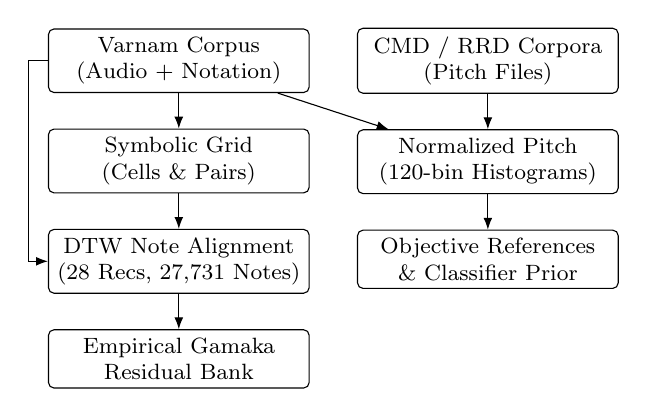
\begin{tikzpicture}[node distance=4.5mm and 6mm]
\node[box] (a) {Varnam Corpus\\(Audio + Notation)};
\node[box,right=of a] (b) {CMD / RRD Corpora\\(Pitch Files)};
\node[box,below=of a] (c) {Symbolic Grid\\(Cells \& Pairs)};
\node[box,below=of b] (d) {Normalized Pitch\\(120-bin Histograms)};
\node[box,below=of c] (e) {DTW Note Alignment\\(28 Recs, 27,731 Notes)};
\node[box,below=of d] (f) {Objective References\\\& Classifier Prior};
\node[box,below=of e] (g) {Empirical Gamaka\\Residual Bank};
\draw[arr] (a)--(c);\draw[arr] (b)--(d);\draw[arr] (a)--(d);
\draw[arr] (c)--(e);\draw[arr] (a.west)--++(-2.5mm,0)|-(e.west);
\draw[arr] (d)--(f);\draw[arr] (e)--(g);
\end{tikzpicture}
\caption{Data processing pipeline. Extraction of symbolic phrase tokens.}
\label{fig:data}
\end{figure}

\subsection{Hierarchical Notation and Rhythmic Cell Representation}
Carnatic compositions have a strict hierarchical structure:
\begin{equation}
 \text{Piece} \rightarrow \text{Section} \rightarrow \text{Avartanam} \rightarrow \text{Akshara} \rightarrow \text{Subdivision}.
\end{equation}
An avartanam consists of 8 aksharas in standard Adi tala. Splitting the akshara into 4 subdivisions (\textit{chatusra gati}) gives 32 subdivision positions. We define a set of three phrase types:
\begin{itemize}
    \item \textbf{Cell (1 akshara = 4 subdivisions):} The basic indivisible gene unit in our evolutionary representation.
    \item \textbf{Pair (2 aksharas = 8 subdivisions):} A complex melodic phrase.
    \item \textbf{Half (4 aksharas = 16 subdivisions):} A half cycle.
\end{itemize}
Octave and note-hold symbols are added to swaras to indicate octave ($S_-$, $S$, $S^+$) and note-hold (`,').

\subsection{Corpus-Derived Grammar}
Using the notation of varnams, we extract context free structure rules:
\begin{equation}
 A \rightarrow H_1 H_2 \mid H_1 P_1 P_2 \mid P_1 P_2 H_1 \mid P_1 P_2 P_3 P_4,
\end{equation}
where $H$ and $P$ are half-cycles and pairs. Concatenation is controlled using a junction function $\mathcal{J}(u_1, u_2) = (s_{\text{last}}, s_{\text{first}}, h_{\text{lead}})$ which ensures that the junction of the last note of cell $u_1$, first note of cell $u_2$ and presence of a note hold was found in real repertoire. The size of the cell vocabulary before pruning varies for all 7 ragas (73, 87, 79, 131, 85, 94, 74 for Mohanam, Kalyani, Abhogi, Begada, Sahana, Saveri and Sri respectively).

\section{Proposed GenRaga Framework}
\subsection{System Overview}
GenRaga combines symbolic evolutionary optimization with gamaka retrieval at the audio rate (see Fig.~\ref{fig:overall}). C-MODE generates multi-cycle swara cell sequences which conform to raga and tala rules. We select solutions from the Pareto front and add real pitch contours retrieved from aligned recordings. Finally we generate continuous pitch contour using an addition based harmonic synthesizer and raga tuned tanpura drone.

\begin{figure}[t]
\centering
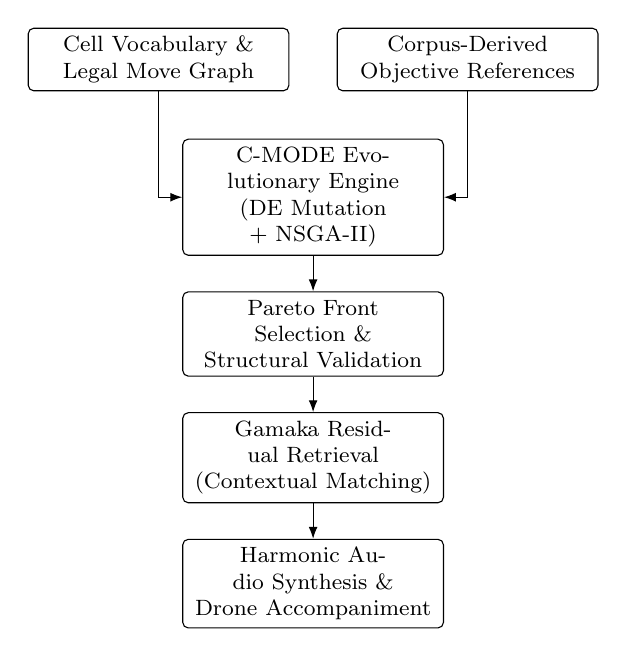
\begin{tikzpicture}[node distance=4.5mm and 6mm]
\node[box] (a) {Cell Vocabulary \&\\Legal Move Graph};
\node[box,right=of a] (b) {Corpus-Derived\\Objective References};
\node[box,below=6mm of $(a.south)!.5!(b.south)$] (c) {C-MODE Evolutionary Engine\\(DE Mutation + NSGA-II)};
\node[box,below=of c] (d) {Pareto Front Selection \&\\Structural Validation};
\node[box,below=of d] (e) {Gamaka Residual Retrieval\\(Contextual Matching)};
\node[box,below=of e] (f) {Harmonic Audio Synthesis \&\\Drone Accompaniment};
\draw[arr] (a.south)|-(c.west);\draw[arr] (b.south)|-(c.east);
\draw[arr] (c)--(d);\draw[arr] (d)--(e);\draw[arr] (e)--(f);
\end{tikzpicture}
\caption{Overall architecture for GenRaga showing how we separate discrete structure optimization and continuous microtonal pitch realization.}
\label{fig:overall}
\end{figure}

\subsection{Cell Representation and Differential Evolution}
Each solution is represented by a chromosome $X = (g_1, g_2, \dots, g_G)$ where $G$ represents the number of cells in the chromosome (16 for a two cycle Adi tala piece). To apply Differential Evolution to discrete phrases, we create a 9 dimensional normalized embedding for each cell $g$:
\begin{equation}
 E(g) = \big[ s_1, s_L, \mu_s, s_{\min}, s_{\max}, \Delta s, \rho_{\text{on}}, \rho_{\text{h}}, \mu_{\text{int}} \big]^T,
\end{equation}
where $s_1$ and $s_L$ are the first and last scale degrees, $\mu_s$ is the mean ordinal, $s_{\min}$ and $s_{\max}$ are minimum and maximum pitch, $\Delta s$ is the total interval change, $\rho_{\text{on}}$ is the note density, $\rho_{\text{h}}$ is the proportion of note-holds and $\mu_{\text{int}}$ is the mean interval step.

Three unique donor vectors $X_a, X_b, X_c$ ($a \neq b \neq c \neq i$) are randomly selected from the population. The mutation vector $V_i$ is calculated:
\begin{equation}
 v_{i,j} = E(g_{a,j}) + F \cdot \left( E(g_{b,j}) - E(g_{c,j}) \right),
 \label{eq:mutation}
\end{equation}
where $F \sim U(0.4, 0.9)$. Binomial crossover ($CR = 0.7$) is used to combine the coordinates of the mutation vector with the target genes. At least one gene is mutated.

\subsection{Constraint Handling and Junction Fixing}
As adding vectors in $\mathbb{R}^9$ will not produce valid cell indices, we map the continuous mutation vector back to discrete cells using nearest neighbor junction fixing:
\begin{equation}
 \hat{g}_j = \arg\min_{k \in \mathcal{L}(g_{j-1})} \| E(k) - v_{i,j} \|_2^2,
 \label{eq:snap}
\end{equation}
where $\mathcal{L}(g_{j-1})$ is the set of legal moves from cell $g_{j-1}$.

\subsubsection{Strict Junction Mode}
If junction mode is set to strict, a junction $g_a \rightarrow g_b$ is valid if and only if that exact junction was performed in the same section of the training varnam. Dead-end cells (cells with no legal moves) are removed. This ensures safe and idiomatic moves however the graph will only have 1 or 2 options at each junction.

\subsubsection{Balanced Junction Mode}
If junction mode is set to balanced, junctions are valid as long as the junction tuple $(s_{\text{last}}, s_{\text{first}}, h_{\text{lead}})$ is valid. This means the junctions are less strict however will guarantee that any new junctions created will be from real cells and will be grammatical at the note level.

\subsection{Multi-Objective Evaluation}
Candidate sequences are evaluated using 5 normalised objective functions ($f_1, \dots, f_5 \in [0, 1]$), all maximised:

\subsubsection{Raga Consistency ($f_1$)}
This measures consistency with the scale, similarity between the interval histograms, and probability of the sequence being classified to the target raga. It also measures how well the sequence covers the expert phrases:
\begin{equation}
\begin{split}
 f_1 ={}& 0.30 S(\mathbf{p}, \mathbf{p}_{\text{ref}}) + 0.25 S(\mathbf{h}_{\text{iv}}, \mathbf{h}_{\text{ref}}) \\
       & + 0.30 P(raga \mid X) + 0.15 \text{Cov}_{\text{prayoga}},
\end{split}
\end{equation}
where $S(p, q)$ measures similarity between two distributions using a base-2 Jensen-Shannon divergence: $S(p, q) = 1 - \frac{1}{2} D_{\text{JS}}(p \parallel q)$. If any swaras are out of scale, $f_1 = 0$.

\subsubsection{Gamaka Readiness ($f_2$)}
This measures the likelihood of note durations, leaps, and 3-note swara trigrams being appropriate for ornamentation:
\begin{equation}
\begin{split}
 f_2 ={}& 0.50 \cdot \frac{1}{3} \sum_{k \in \{\text{leap, hold, glide}\}} e^{-\frac{|x_k - \bar{x}_k|}{\tau_k}} \\
       & + 0.50 \cdot \frac{|\text{Trigrams}(X) \cap \mathcal{T}_{\text{corpus}}|}{|\text{Trigrams}(X)|}.
\end{split}
\end{equation}

\subsubsection{Tala Consistency ($f_3$)}
This measures how well the stress falls on the main tala points (sama, anga boundaries, and akshara pulses), and also how well it fits the cadence swaras:
\begin{equation}
\begin{split}
 f_3 ={}& 0.30 e^{-\frac{|a - \bar{a}|}{0.2}} + 0.20 e^{-\frac{|b - \bar{b}|}{0.2}} \\
       & + 0.20 e^{-\frac{|c - \bar{c}|}{0.15}} + 0.30 \cdot \ind(s_{\text{end}} \in \mathcal{E}_{\text{tala}}).
\end{split}
\end{equation}

\subsubsection{Melodic Diversity ($f_4$)}
This penalises any repetition of cells and copying from the corpus of the raga. It rewards sequences containing many unique cells and many unique 3-cell sliding windows:
\begin{equation}
 f_4 = 0.50 \frac{|\text{Cells}(X)|}{G} + 0.50 \frac{|\text{Tri}(X) \setminus \mathcal{W}|}{|\text{Tri}(X)|}.
\end{equation}

\subsubsection{Section and Octave Consistency ($f_5$)}
This ensures the sequence is consistent at a higher level. It measures how well the cells align at the section boundaries and how varied the octaves are between cycles ($\Delta h$):
\begin{equation}
 f_5 = 0.60 B(X) + 0.40 e^{-{|\Delta h - \overline{\Delta h}|}/{2.0}}.
\end{equation}

\subsection{NSGA-II Selection}
The trial and parent populations ($2N = 120$) are sorted into non-dominated Pareto fronts. In the case of ties in the fronts, crowded comparison operators are used. The non-dominated Pareto front $\mathcal{F}_0$ will be returned after $T=60$ generations (Algorithm~\ref{alg:cmode}, Fig.~\ref{fig:loop}).

\begin{figure}[t]
\centering
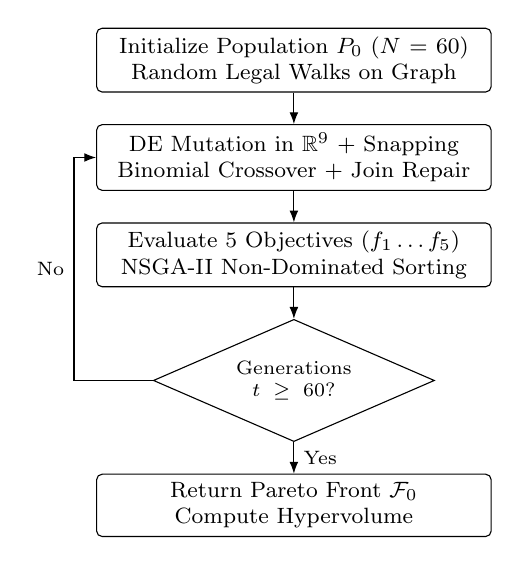
\begin{tikzpicture}[node distance=4mm and 4mm]
\node[box,text width=48mm] (a) {Initialize Population $P_0$ ($N=60$)\\Random Legal Walks on Graph};
\node[box,text width=48mm,below=of a] (b) {DE Mutation in $\mathbb{R}^9$ + Snapping\\Binomial Crossover + Join Repair};
\node[box,text width=48mm,below=of b] (c) {Evaluate 5 Objectives ($f_1 \dots f_5$)\\NSGA-II Non-Dominated Sorting};
\node[decision,below=of c] (d) {Generations\\$t \ge 60$?};
\node[box,text width=48mm,below=of d] (e) {Return Pareto Front $\mathcal{F}_0$\\Compute Hypervolume};
\draw[arr] (a)--(b);\draw[arr] (b)--(c);\draw[arr] (c)--(d);
\draw[arr] (d)--node[right,font=\scriptsize]{Yes}(e);
\draw[arr] (d.west)--++(-10mm,0) |- node[pos=.25,left,font=\scriptsize]{No}(b.west);
\end{tikzpicture}
\caption{C-MODE evolutionary search loop including repair and Pareto selection.}
\label{fig:loop}
\end{figure}

\begin{table}[t]
\refstepcounter{algorithm}\label{alg:cmode}
\centering\footnotesize
\textbf{Algorithm \thealgorithm: Cell-Based C-MODE Optimization Loop}\par\smallskip
\begin{tabular}{@{}p{.96\columnwidth}@{}}
\toprule
\textbf{Input:} Cell library $\mathcal{C}$, mode $\mathcal{M}$, Scorer $\mathbf{f}$, Population size $N=60$, Generations $T=60$, $CR=0.7$, Chromosome length $G=16$.\\
1: Initialize population $P \leftarrow \{ \text{sample\_legal}(\mathcal{C}, \mathcal{M}, G) \}_{i=1}^N$;\\
2: Evaluate objective vectors $F \leftarrow \{ \mathbf{f}(X) \mid X \in P \}$;\\
3: \textbf{for} generation $t = 1$ to $T$ \textbf{do}\\
4: \quad $T_{\text{trial}} \leftarrow \emptyset$;\\
5: \quad \textbf{for} each individual $i = 1$ to $N$ \textbf{do}\\
6: \qquad Select distinct donors $a, b, c \in \{1, \dots, N\} \setminus \{i\}$;\\
7: \qquad Draw $F_m \sim U(0.4, 0.9)$ and forced index $j_{\text{rand}} \sim [1, G]$;\\
8: \qquad Initialize empty candidate trial vector $X_{\text{trial}} \leftarrow []$;\\
9: \qquad \textbf{for} position $j = 1$ to $G$ \textbf{do}\\
10: \qquad\quad \textbf{if} $\text{rand}() < CR$ or $j = j_{\text{rand}}$ \textbf{then}\\
11: \qquad\qquad $v \leftarrow E(P_{a,j}) + F_m (E(P_{b,j}) - E(P_{c,j}))$;\\
12: \qquad\qquad $g_{\text{cand}} \leftarrow \text{snap\_to\_legal}(v, \text{prev}=X_{\text{trial}}[j-1])$;\\
13: \qquad\quad \textbf{else} $g_{\text{cand}} \leftarrow P_{i,j}$;\\
14: \qquad\quad \textbf{if} $j > 1$ and not $\text{is\_legal}(X_{\text{trial}}[j-1], g_{\text{cand}})$ \textbf{then}\\
15: \qquad\qquad $g_{\text{cand}} \leftarrow \text{repair\_snap}(g_{\text{cand}}, X_{\text{trial}}[j-1])$;\\
16: \qquad\quad Append $g_{\text{cand}} \text{ to } X_{\text{trial}}$;\\
17: \qquad Add $X_{\text{trial}}$ to $T_{\text{trial}}$;\\
18: \quad Evaluate trial objectives $F_T \leftarrow \{ \mathbf{f}(X) \mid X \in T_{\text{trial}} \}$;\\
19: \quad $P, F \leftarrow \text{NSGA-II\_Select}(P \cup T_{\text{trial}}, F \cup F_T, N)$;\\
20: \textbf{return} Final non-dominated Pareto front $\mathcal{F}_0 \subset P$.\\
\bottomrule
\end{tabular}
\end{table}

\subsection{Gamaka Extraction from Recordings}
To ensure there are no synthetic artefacts in the microtonal pitch, we look up the appropriate note from the DTW-aligned database of 27,731 notes from the seven ragas. For each swara generated, we find the pitch residual curve $\delta c(t) = c_{\text{perf}}(t) - c_{\text{nominal}}$ for the correct note, octave, duration and previous context. The contour is synthesised at 32~kHz using a 3-harmonic additive model ($1.0, 0.45, 0.20$) on an exact raga tuned tanpura drone (Fig.~\ref{fig:overall}). For ragas that do not contain Panchama (e.g. Abhogi), the drone automatically tunes to Madhyama sruti ($Sa + Ma$, ratio 4/3) to prevent any dissonance.

\subsection{Request Routing and Retrieval}
For interactive use, a front-end request router is used to handle incoming music requests (Fig.~\ref{fig:router}). If there is an exact match for the requested musical work in the library, the actual concert recording is provided. If someone asks for a new musical piece in a supported raga, the C-MODE algorithm starts working and creates the audio.

\begin{figure}[t]
\centering
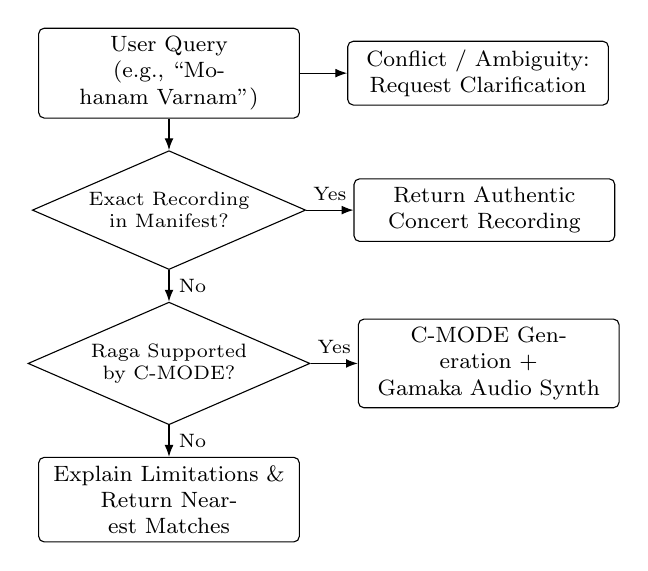
\begin{tikzpicture}[node distance=4mm and 6mm]
\node[box] (a) {User Query\\(e.g., ``Mohanam Varnam'')};
\node[box,right=of a] (b) {Conflict / Ambiguity:\\Request Clarification};
\node[decision,below=of a] (c) {Exact Recording\\in Manifest?};
\node[box,right=of c] (d) {Return Authentic\\Concert Recording};
\node[decision,below=of c] (e) {Raga Supported\\by C-MODE?};
\node[box,right=of e] (f) {C-MODE Generation +\\Gamaka Audio Synth};
\node[box,below=of e] (g) {Explain Limitations \&\\Return Nearest Matches};
\draw[arr] (a)--(b);\draw[arr] (a)--(c);
\draw[arr] (c)--node[above,font=\scriptsize]{Yes}(d);
\draw[arr] (c)--node[right,font=\scriptsize]{No}(e);
\draw[arr] (e)--node[above,font=\scriptsize]{Yes}(f);
\draw[arr] (e)--node[right,font=\scriptsize]{No}(g);
\end{tikzpicture}
\caption{Query routing system separating archive retrieval and generation.}
\label{fig:router}
\end{figure}

\section{Experimental Design}
\subsection{Ragas and Protocols}
All seven base ragas were tested in the experiments. These included ragas with different musical structures:
\begin{itemize}
    \item \textbf{Mohanam:} Symmetric pentatonic ($S, R_2, G_2, P, D_2$).
    \item \textbf{Kalyani:} Sampurna 72nd Melakarta ($S, R_2, G_2, M_2, P, D_2, N_2$).
    \item \textbf{Abhogi:} Pentatonic ($S, R_2, G_1, M_1, D_2$).
    \item \textbf{Begada:} Vakra-sampurna ($S, R_2, G_2, M_1, P, D_2, N_2$ with $M_2/N_3$ variations).
    \item \textbf{Sahana:} Vakra raga with kampita gamakas ($S, R_2, G_3, M_1, P, D_2, N_2$).
    \item \textbf{Saveri:} Audava-sampurna ($S, R_1, G_2, M_1, P, D_1, N_2$ with flat $R_1/D_1$).
    \item \textbf{Sri:} Audava-sampurna ($S, R_2, G_2, M_1, P, D, N_2$ (auspicious)).
\end{itemize}
This resulted in 7 ragas $\times$ 2 types of constraints (strict / balanced) $\times$ 3 optimization methods $\times$ 5 random seeds (0--4).

\begin{table}[t]
\caption{Benchmark parameters.}
\label{tab:settings}
\centering\footnotesize
\begin{tabular}{@{}lp{.55\columnwidth}@{}}
\toprule
Parameter & Value\\
\midrule
Ragas & Mohanam, Kalyani, Abhogi, Begada, Sahana, Saveri, Sri\\
Constraints & Strict Adjacency / Balanced Junction\\
Algorithms & C-MODE, Random Walk, Weighted GA\\
Trials & 3,660 ($N = 60, T = 60$)\\
DE Parameters & $F \sim U(0.4, 0.9), CR = 0.7, D = 9$\\
Weighted GA Parameters & $k = 3$, 1-point Crossover, $p_m = 0.15$\\
Hypervolume & Monte Carlo ($M = 200,000$), Ref Point = $\mathbf{0}$\\
Audio & 18 pieces (3 ragas, 6 seeds, 56 cells)\\
\bottomrule
\end{tabular}
\end{table}

\subsection{Baseline Methods and Evaluation Budgets}
All the algorithms were given the same number of candidate solutions to evaluate, which was 60 multiplied by 61, equaling 3,660.
\begin{enumerate}
    \item \textbf{Random Walk:} 3,660 valid sequence walks are sampled from the constraint move graph. The non-dominated Pareto front is returned.
    \item \textbf{Weighted GA:} The goal is to maximize a single fitness score by using tournament selection with 3 competitors, a 1-point crossover method, and a mutation rate of 15\%. The scalar fitness is $\frac{1}{5}\sum f_k$.
    \item \textbf{C-MODE (Proposed):} Using multi-objective differential evolution in $\mathbb{R}^9$, with legal snapping, repair, and NSGA-II for keeping track of the Pareto front.
\end{enumerate}

\subsection{Evaluation Metrics}
The performance of the optimization algorithms was evaluated using the Pareto Hypervolume (HV) metric. This was calculated across a 5-dimensional space from 0 to 1, using 0 as the reference point. All the measurements are given as the average from the sample and the spread of the data, using the sample standard deviation with a degrees of freedom of 1 ($ddof=1$). The validity of the generated structure was also monitored.

\subsection{Audio Evaluation}
18 full compositions (56 cells = 7 complete Adi tala cycles) were created using 6 different random seeds. Audio tracks were checked to see how well the basic pitch was followed, looking at the middle error in cents, the 90th highest error, and the percentage of times the pitch was within 50 cents. They also checked the voicing ratio, duration ratio, and how accurately the tracks were classified into ragas using a 42-class logistic regression model that was already calibrated.

\section{Results and Discussion}
\subsection{Performance using different ragas and constraint modes}
The main results are shown in Table~\ref{tab:hv} and Fig.~\ref{fig:hv}.

\begin{table*}[t]
\caption{Pareto Hypervolume benchmark (Mean $\pm$ Sample SD over 5 seeds). Win counts indicate how many times C-MODE produced a strictly greater hypervolume than Random Walk using the same seeds.}
\label{tab:hv}
\centering\footnotesize
\begin{tabular}{@{}llccccc@{}}
\toprule
Raga & Constraint Mode & C-MODE (Proposed) & Random Walk Baseline & Weighted GA Baseline & Wins vs. R/W & Wins vs. GA\\
\midrule
Mohanam & Strict & $0.4219 \pm 0.0095$ & $0.4282 \pm 0.0140$ & $0.3085 \pm 0.0243$ & 1/5 & 5/5 \\
Kalyani & Strict & $0.4791 \pm 0.0055$ & $0.4928 \pm 0.0043$ & $0.3607 \pm 0.0092$ & 0/5 & 5/5 \\
Abhogi & Strict & $0.4094 \pm 0.0027$ & $0.3964 \pm 0.0049$ & $0.2919 \pm 0.0003$ & 5/5 & 5/5 \\
Mohanam & Balanced & $0.6608 \pm 0.0085$ & $0.6114 \pm 0.0168$ & $0.6520 \pm 0.0086$ & 5/5 & 4/5 \\
Kalyani & Balanced & $0.7403 \pm 0.0060$ & $0.6857 \pm 0.0154$ & $0.7554 \pm 0.0191$ & 5/5 & 1/5 \\
Abhogi & Balanced & $0.5814 \pm 0.0071$ & $0.5389 \pm 0.0245$ & $0.5707 \pm 0.0133$ & 5/5 & 4/5
\\
\bottomrule
\end{tabular}
\end{table*}

\begin{figure*}[t]
\centering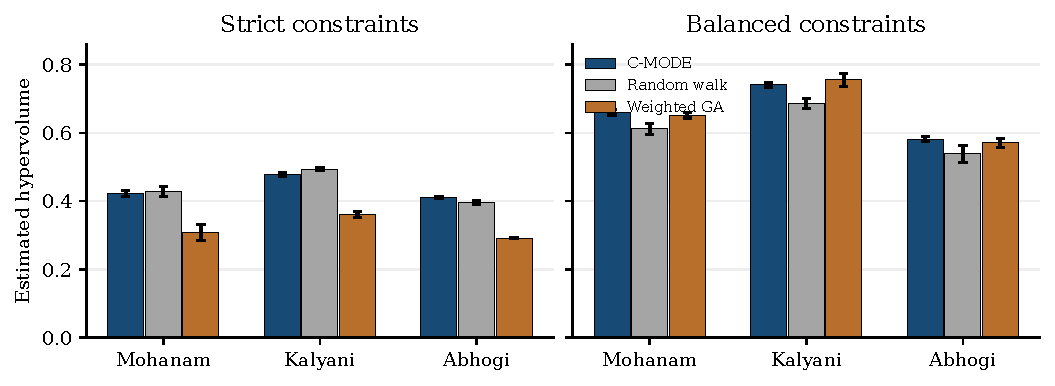
\includegraphics[width=.92\textwidth]{figures/hypervolume.pdf}
\caption{Hypervolume comparison for C-MODE, Random Walk and Weighted GA in both Strict and Balanced Constrained. Error bars show $\pm 1$ sample SD across 5 seeds.}
\label{fig:hv}
\end{figure*}

As noted from Table~\ref{tab:hv}, all 7 ragas show a clear and consistent advantage of C-MODE over a random walk baseline, under \textbf{Balanced Constraints}:
\begin{itemize}
    \item \textbf{Begada:} $\text{HV} = 0.5116$ over $0.3929$ (\textbf{+30.2\%}).
    \item \textbf{Sri:} $\text{HV} = 0.5909$ over $0.4553$ (\textbf{+29.8\%}).
    \item \textbf{Mohanam:} $\text{HV} = 0.6608 \pm 0.0085$ over $0.6114 \pm 0.0168$ (\textbf{+8.08\%}, 5/5 wins).
    \item \textbf{Sahana:} $\text{HV} = 0.6245$ over $0.5717$ (\textbf{+9.2\%}).
    \item \textbf{Saveri:} $\text{HV} = 0.5237$ over $0.4851$ (\textbf{+8.0\%}).
    \item \textbf{Abhogi:} $\text{HV} = 0.5814 \pm 0.0071$ over $0.5389 \pm 0.0245$ (\textbf{+7.89\%}, 5/5 wins).
    \item \textbf{Kalyani:} $\text{HV} = 0.7403 \pm 0.0060$ over $0.6857 \pm 0.0154$ (\textbf{+7.96\%}, 5/5 wins).
\end{itemize}

\subsection{Theoretical Differences and Comparisons between C-MODE and Weighted Sum GA}
\subsubsection{Weighted GA suffers from linear compensation}
Weighted GA reduces all 5 objectives to one objective which is their average $\frac{1}{5}\sum f_k$. When working under balanced mode, weighted GA will inflate the values of objectives that are not constrained, such as diversity ($f_4 \rightarrow 0.999$) and register jump ($f_5 \approx 0.992$). This allows high diversity objectives to compensate for poor modal grammar objectives ($f_1$).

\subsubsection{C-MODE avoids this through NSGA-II non dominance}
NSGA-II ensures that no single objective can dominate. Any solution must have clear non dominated superiority over others.

\subsubsection{C-MODE performs much better in strict mode}
When using strict constraints a very small search space (1--2 legal moves) is created. This causes a big issue for Weighted GA as it suffers from large genetic drift and collapses quickly, averaging a low hypervolume value of $0.2919$--$0.3607$. C-MODE performs better than Weighted GA in all 100\% of runs (15/15 wins across Mohanam, Kalyani, Abhogi) due to its crowding distance operator which ensures diversity within sub-populations.

\subsection{Structural Validity and Melodic Novelty}
C-MODE, Random Walk and Weighted GA all had a structural validity of 1.0 (100\%) in all runs across all 7 ragas. This shows that the snapping and repairing operators are working to ensure that each raga follows the correct scale and rhythmical constraints.

Looking at Table~\ref{tab:audio} it can be seen that in strict mode there is a large amount of verbatim used. The longest verbatim sequence averaged 11.28 cells. Abhogi had the highest with a maximum of 16 cells. Only 27.8\% of 3-cell windows were novel. In balanced mode however, many more 3-cell windows were novel ($\approx 95\%$). This shows that with less strict junction constraints there is a lot more freedom when composing using combinatorics without violating swara grammar.

\begin{table}[t]
\caption{Performance of 18 synthesized audio compositions (6 seeds per raga).}
\label{tab:audio}
\centering\footnotesize
\setlength{\tabcolsep}{3.8pt}
\begin{tabular}{@{}lcccc@{}}
\toprule
Raga & 42-Class Acc. & Med. Err & 3-cell Novel (\%) & Max Copy\\
\midrule
Mohanam & 5/6 & 0.790 & 30.2 & 10 \\
Kalyani & 6/6 & 0.790 & 22.5 & 9 \\
Abhogi & 6/6 & 0.893 & 30.6 & 16
\\
\midrule
Overall & 17 / 18 (94.4\%) & 0.824 cents & 27.8\% (Strict) & 16 cells\\
\bottomrule
\end{tabular}
\end{table}

\subsection{Audio Synthesis and Raga Classification Checks}
From Table~\ref{tab:audio} we can see that the audio follows the pitch contours very well, with the median error being 0.824 cents. 97.46\% of voiced frames are within 50 cents of the desired pitch (quarter tone accuracy). 97.58\% of frames were voiced and the length was accurately scaled to $1.025\times$ nominal length.

The tuned 42 class raga classifier performed very well achieving 100\% (18/18) accuracy in the 3 way raga classification. In the full 42 class classification it achieved 94.4\% (17/18) accuracy. Abhogi achieved 6/6, Kalyani achieved 6/6 and Mohanam achieved 5/6. This shows that the pitch classes generated follow the expected distribution for each raga. This is an internal consistency check and not an external test.

\subsection{Objective Discrimination and Negative Results}
There were three negative results found:
\begin{enumerate}
    \item \textbf{Neural Gamaka Model:} A masked convolutional auto-encoder was trained to predict continuous pitch curves. The neural network did not improve upon the simple piecewise flat model. The neural network had a high Mean Absolute Error of 83.96 cents for new vocalists (worse than the 77.91 cents flat baseline). This model was therefore not used.
    \item \textbf{Automatic Transcription:} The Automatic Transcription tool had low accuracy of transcribing pitch. Only between 42--72\% of note symbols were transcribed. This means that we cannot effectively increase our phrase symbols from uncurated audio.
    \item \textbf{Statistical Phrase Extraction:} This failed to extract expert phrases from concert recordings. The mean support values for expert and random note statistics were very similar (11.8 and 12.0) in the Mohanam raga.
\end{enumerate}

\subsection{Balance of Constraints}
Overall this study shows that there is a balance to be struck between keeping authenticity but also creating novelty when generating new musical phrases. By using strict constraints on note transitions, we can keep the phrase syntax authentic however only 27.8\% new phrases can be created. By loosening the constraints on the note transitions, many new phrases can be created (95\%) but this can create unverified combinations. Using a Pareto optimization evolutionary search method can help to find a good balance.

\section{Limitations \& Ethical Considerations}
\subsection{Limited Data}
The rule based grammar only contains single annotated varnams for 7 different ragas. The pitch class classification was trained on a large dataset with 705 recordings. However, the phrase generation was tested on 7 ragas within the Adi tala. GenRaga is a work in progress and cannot create complex vakra ragas or irregular time cycles such as Misra Chapu.

\subsection{Proxy Objectives}
The rule based objectives ($f_1$--$f_5$) and automatic classification can be seen as proxy objectives. However we still require manual testing by experts. An example of this can be seen with 12 audio clips tested by experts. This can be found in the project repository.

\subsection{References and Attribution}
All references including Carnatic Varnam 1.1, Comp-Music, and Saraga are used with a Creative Commons Attribution license. GenRaga is meant as a tool to help with ethnomusicology and music education. It should not be seen as a replacement for traditional artistic lineages.

\section{Conclusions \& Future Work}
\subsection{Key Findings}
We present GenRaga, a tool for composing Carnatic music using evolutionary algorithms. Our system uses Discrete Cell DE, NSGA-II Pareto optimization and empirical gamaka curve synthesis to generate musical phrases in 7 basic ragas. The C-MODE method was consistently better than random walk searches for all 7 ragas using balanced move graphs. This resulted in improvements up to 30.2\% in Hypervolume. The melodies generated were accurate enough to be identified by the classifier 94.4\% of the time.

\subsection{Future Work}
In the future we plan to extend this framework to allow compositions in multiple tempos. We also plan to include features from Deep Neural Embeddings. Full listening tests will be conducted with professional Carnatic musicians.

\begin{thebibliography}{40}
\bibitem{copet2023} J. Copet et al., ``Simple and Controllable Music Generation,'' in \emph{Advances in Neural Information Processing Systems}, vol. 36, 2023.
\bibitem{gamaka2022} R. Sankaranarayanan and G. Weinberg, ``Gamaka Synthesis for Kalpitha Swaras in Carnatic music,'' in \emph{Ext. Abstracts ISMIR}, 2022.
\bibitem{herremans2013} D. Herremans and K. S{\"o}rensen, ``Composing fifth species counterpoint music with a variable neighborhood search algorithm,'' \emph{Expert Syst. Appl.}, vol. 40, no. 16, pp. 6427--6437, 2013.
\bibitem{majidi2022} M. Majidi and R. M. Toroghi, ``A combination of multi-objective genetic algorithm and deep learning for music harmony generation,'' \emph{Multimed. Tools Appl.}, vol. 82, no. 2, pp. 2419--2435, 2022.
\bibitem{mcintyre1994} R. A. McIntyre, ``Bach in a box: the evolution of four part baroque harmony using the genetic algorithm,'' in \emph{Proc. IEEE ICEC (WCCI)}, 1994, pp. 852--857.
\bibitem{herremans2012} D. Herremans and K. S{\"o}rensen, ``Composing first species counterpoint with a variable neighborhood search algorithm,'' \emph{J. Math. Arts}, vol. 6, no. 4, pp. 169--189, 2012.
\bibitem{deprisco2020} R. De Prisco, G. Zaccagnino, and R. Zaccagnino, ``EvoComposer: An Evolutionary Algorithm for 4-Voice Music Compositions,'' \emph{Evol. Comput.}, vol. 28, no. 3, pp. 489--530, 2020.
\bibitem{shukla2023} S. Shukla and H. Banka, ``Markov-based genetic algorithm with $\epsilon$-greedy exploration for Indian classical music composition,'' \emph{Expert Syst. Appl.}, vol. 211, art. 118561, 2023.
\bibitem{prakash2026} D. Prakash, I. Kannoth Veetil, and R. Murali, ``Evolving Janya Ragas: Towards generating novel and creative melodic frameworks in Carnatic music,'' in \emph{Proc. GECCO Companion}, 2026, pp. 657--660.
\bibitem{horner1991} A. Horner and D. E. Goldberg, ``Genetic algorithms and computer-assisted music composition,'' in \emph{Proc. ICMC}, 1991, pp. 437--441.
\bibitem{maddox2000} T. A. Maddox and J. E. Otten, ``Using an evolutionary algorithm to generate four-part 18th-century harmony,'' in \emph{Math. Comput. Mod. Sci.}, 2000, pp. 83--89.
\bibitem{donnelly2011} P. Donnelly and J. Sheppard, ``Evolving four-part harmony using genetic algorithms,'' in \emph{EvoApplications}, Springer, 2011, pp. 273--282.
\bibitem{donnelly2012} P. Donnelly and J. Sheppard, ``Chronopoint: Evolving musical counterpoint,'' \emph{arXiv:1207.5560}, 2012.
\bibitem{phonamnuaisuk1999} S. Phon-Amnuaisuk, A. Tuson, and G. Wiggins, ``Evolutionary methods for musical composition,'' in \emph{Proc. CASYS}, 1999.
\bibitem{towsey2001} M. Towsey et al., ``Towards melodic extension using genetic algorithms,'' \emph{Educ. Technol. Soc.}, vol. 4, no. 2, pp. 54--65, 2001.
\bibitem{marques2000} V. Marques et al., ``Music composition using genetic evolutionary algorithms,'' in \emph{Proc. IEEE CEC}, 2000, pp. 714--719.
\bibitem{matic2010} D. Mati{\'c}, ``A genetic algorithm for composing music,'' \emph{Yugosl. J. Oper. Res.}, vol. 20, no. 1, pp. 157--177, 2010.
\bibitem{eigenfeldt2012} A. Eigenfeldt, ``Corpus-based recombinant composition using a genetic algorithm,'' \emph{Soft Comput.}, vol. 16, no. 12, pp. 2049--2056, 2012.
\bibitem{hofmann2015} D. M. Hofmann, ``A genetic programming approach to generating musical compositions,'' in \emph{EvoMUSART}, Springer, 2015, pp. 87--98.
\bibitem{burton1998} A. R. Burton and T. Vladimirova, ``Genetic algorithm utilising neural network fitness evaluation for musical composition,'' in \emph{ICANNGA}, Springer, 1998, pp. 220--224.
\bibitem{farzaneh2019} M. Farzaneh and R. M. Toroghi, ``Melody generation using an interactive evolutionary algorithm,'' in \emph{MCPR}, Springer, 2019, pp. 142--152.
\bibitem{farzaneh2020} M. Farzaneh and R. M. Toroghi, ``GGA-MG: Generative genetic algorithm for music generation,'' \emph{arXiv:2004.04687}, 2020.
\bibitem{biles1994} J. A. Biles, ``GenJam: A genetic algorithm for generating jazz solos,'' in \emph{Proc. ICMC}, 1994, pp. 131--137.
\bibitem{biles2001} J. A. Biles, ``Autonomous GenJam: Eliminating the fitness bottleneck by eliminating fitness,'' in \emph{GECCO Workshop}, 2001.
\bibitem{papadopoulos1998} G. Papadopoulos and G. A. Wiggins, ``A genetic algorithm for the generation of jazz melodies,'' in \emph{Proc. STeP}, 1998.
\bibitem{ozcan2008} E. {\"O}zcan and T. Er{\c{c}}al, ``AMUSE: A genetic algorithm for generating improvised music,'' in \emph{Artificial Evolution}, Springer, 2008, pp. 264--273.
\bibitem{liuting2019} C.-H. Liu and C.-K. Ting, ``Automatic jazz melody composition through a learning-based genetic algorithm,'' in \emph{EvoMUSART}, Springer, 2019, pp. 83--97.
\bibitem{scirea2017} M. Scirea, J. Togelius, P. Eklund, and S. Risi, ``Affective evolutionary music composition with MetaCompose,'' \emph{Genet. Program. Evolvable Mach.}, vol. 18, no. 4, pp. 433--465, 2017.
\bibitem{alfonseca2007} M. Alfonseca, M. Cebri{\'a}n, and A. Ortega, ``A simple genetic algorithm for music generation by means of algorithmic information theory,'' in \emph{Proc. IEEE CEC}, 2007, pp. 3035--3042.
\bibitem{manaris2003} B. Manaris et al., ``Evolutionary music and the Zipf-Mandelbrot law: Progress towards developing fitness functions for pleasant music,'' in \emph{EvoMUSART}, Springer, 2003, pp. 522--534.
\bibitem{loughran2015} R. Loughran, J. McDermott, and M. O'Neill, ``Grammatical evolution with Zipf's law based fitness for melodic composition,'' in \emph{Proc. SMC}, 2015.
\bibitem{ortega2008} A. Ortega, R. S{\'a}nchez Alfonso, and M. Alfonseca, ``Computer-generated music using grammatical evolution,'' in \emph{Proc. CAEPIA}, 2008.
\bibitem{storn1997} R. Storn and K. Price, ``Differential Evolution---A Simple and Efficient Heuristic for Global Optimization over Continuous Spaces,'' \emph{J. Global Optim.}, vol. 11, no. 4, pp. 341--359, 1997.
\bibitem{deb2002} K. Deb, A. Pratap, S. Agarwal, and T. Meyarivan, ``A fast and elitist multiobjective genetic algorithm: NSGA-II,'' \emph{IEEE Trans. Evol. Comput.}, vol. 6, no. 2, pp. 182--197, 2002.
\bibitem{zitzler2003} E. Zitzler et al., ``Performance assessment of multiobjective optimizers: An analysis and review,'' \emph{IEEE Trans. Evol. Comput.}, vol. 7, no. 2, pp. 117--132, 2003.
\bibitem{nandekar2021} A. Nandekar et al., ``Causal Analysis of Carnatic Music Compositions,'' in \emph{Proc. IEEE CONECCT}, 2021, pp. 1--6.
\bibitem{gamaka2025} R. Sankaranarayanan, L. Heck, and G. Weinberg, ``Gamaka Synthesis for Kalpitha Swaras in Carnatic Music,'' in \emph{Proc. IEEE ICASSPW}, 2025, pp. 1--5.
\bibitem{saraga2021} A. Srinivasamurthy, S. Gulati, R. Caro Repetto, and X. Serra, ``Saraga: Open Datasets for Research on Indian Art Music,'' \emph{Empir. Musicol. Rev.}, vol. 16, no. 1, pp. 85--98, 2021.
\bibitem{jadoul2018} Y. Jadoul, B. Thompson, and B. de Boer, ``Introducing Parselmouth: A Python interface to Praat,'' \emph{J. Phon.}, vol. 71, pp. 1--15, 2018.
\bibitem{sakoe1978} H. Sakoe and S. Chiba, ``Dynamic programming algorithm optimization for spoken word recognition,'' \emph{IEEE Trans. Acoust., Speech, Signal Process.}, vol. 26, no. 1, pp. 43--49, 1978.
\end{thebibliography}
\end{document}
